\documentclass{../presentation}

\usepackage{../Tsinghua}

\title{Leveraging User-Generated Content for Product Promotion: The Effects of Firm-highlighted Reviews}

\author{姚欣培\;王元翔\;钱思涵\;皇甫硕龙}

\begin{document}
    \begin{frame}
        \maketitle
    \end{frame}
    \section{\textsc{Introduction}}
    \begin{frame}
        \frametitle{\textsc{Introduction}}

            \textbf{User-generated content (UGC): }
            \begin{itemize}
                \item blogs, product reviews, and videos...
                \item UGC is often considered more trustworthy than marketer-initiated information (eMarketer 2010, Lee and Koo 2012, Lawrence et al. 2013)
                \item more than 90\% of online customers read reviews before making purchase decisions (eMarketer 2017)
            \end{itemize}

    \end{frame}

    \begin{frame}
        \frametitle{\textsc{Highlighted Reviews and Marketing Effect}}

        \textbf{Highlighted reviews can help firms leverage existing reviews on review platforms}

        \begin{itemize}
            \item highlighting a positive review can potentially attract more attention to the review and lead to more positive product evaluations
            \item may also arouse consumers' skepticism (Settle and Golden 1974, Brown and Krishna 2004) and not achieve the marketing purpose
        \end{itemize}

        Marketing effect of highlighting reviews is affected by

        \textbf{(1)} extremity of review, \textbf{(2)} variance of other reviews and \textbf{(3)} reputation of firm.

    \end{frame}

    \begin{frame}
        \frametitle{\textsc{Model Design}}

        \begin{figure}
            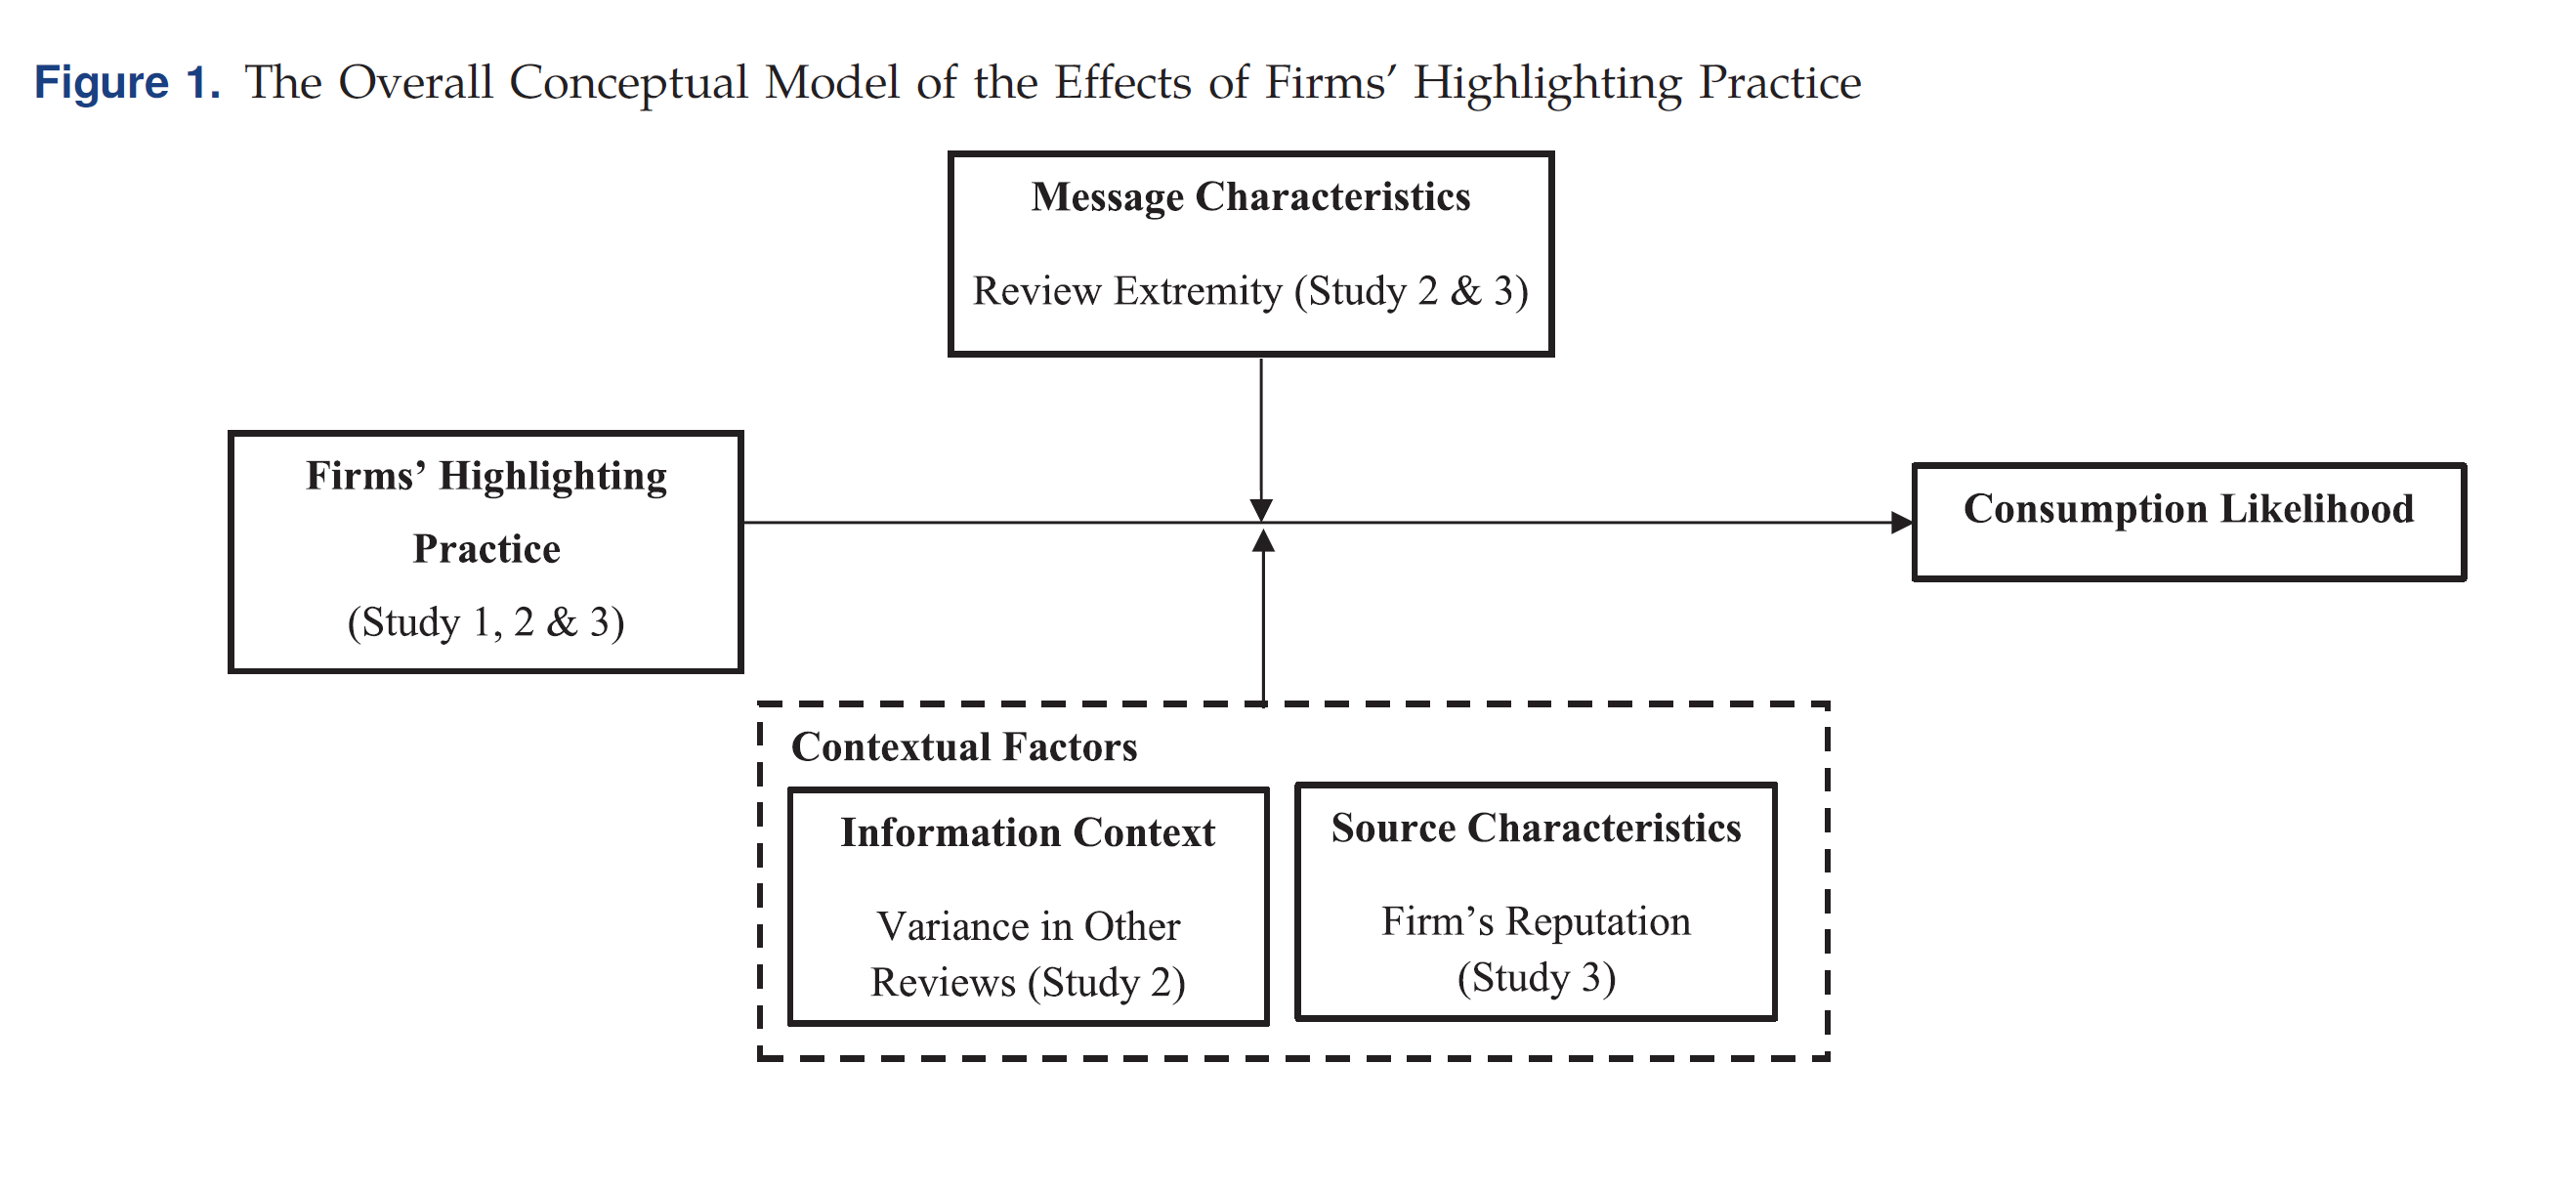
\includegraphics[width=0.9\linewidth]{pre04-imgs/pre04-1.png}
        \end{figure}

    \end{frame}

    \section{\textsc{Research Content}}

    \subsection[\textsc{Study I}]{\textsc{Study I: Salience Effect and Consumers' Skepticism}}

    \begin{frame}
        \frametitle{\textsc{Elevated Skepticism About a Firm-Highlighted Review}}

        \begin{itemize}
            \item The marketing practice of highlighting a positive review may lead to greater attention to this review,
            the elevated consumer skepticism about the firm-highlighted review may offset the intended positive effect of the salient placement of the review.
            \item In contrast, if a positive highlighted review does not arouse consumers' skepticism consumers may accept it at its positive face value.
        \end{itemize}

    \end{frame}

    \begin{frame}
        \frametitle{\textsc{Study I}}

        \begin{itemize}
            \item \textrm{\bfseries Hypothesis 1a:} A review will attract more attention when it is highlighted than when it is not
            \item \textrm{\bfseries Hypothesis 1b:} A positive review will lead to higher consumption likelihood when it is highlighted without and explicit marketing intent than
            \begin{enumerate}
                \item when the review is not highlighted and
                \item when it is highlighted with an explic  marketing intent
            \end{enumerate}
        \end{itemize}

    \end{frame}

    \begin{frame}
        \frametitle{\textsc{Experiment Design}}

        \begin{itemize}
            \item \textbf{Experiment goal: } test the hypothesis using reviews of a restaurant sourced from a major review website
            \item \textbf{Condition settings:}
            \begin{enumerate}
                \item \textbf{Firm-highlighted review} highlighted and labeled with note "\textit{the restaurant paid to highlight this review on top}"
                \item \textbf{Plain highlighted review} highlighted and lebeled with note "\textit{top-placed review}"
                \item \textbf{Baseline} - placed on top but not highlighted or labeled
                \item[*] order of all reviews was the same in the above conditions
            \end{enumerate}
        \end{itemize}

    \end{frame}

    \begin{frame}
        \frametitle{\textsc{Experiment Design}}

        Two effects are evaluated in the experiment

        \begin{itemize}
            \small
            \item \textbf{Salience effect: } plain highlighted review V.S. baseline
            \item \textbf{Consumer skepticism effect: } plain highlighted review V.S. firm-highlighted review
        \end{itemize}

    \end{frame}

    \begin{frame}
        \frametitle{\textsc{Results}}

        Stronger skepticism about the firm-highlighted review than both the plain highlighted review and the normal first review in the baseline condition

        \small
        \setstretch{1.2}

        \begin{enumerate}
            \item The plain highlighted review condition led to higher consumption intention than the baseline as well as the firm-highlighted review condition
            \item The consumption intention in the firm-highlighted review condition did not outperform that in the baseline condition.
        \end{enumerate}

        \begin{itemize}
            \item A salient firm-highlighted review could effectively attract attention, plausibly because it was still a genuine review.
            \item When consumers' skepticism is alleviated, presenting a firm's highlight may exert a positive effect on consumers' likelihood of consumption
        \end{itemize}

    \end{frame}

    \subsection[\textsc{Study II}]{\textsc{Study II: Review Extremity and Variance}}

    \begin{frame}
        \frametitle{\textsc{Information Context - Variance}}

        \small
        \setstretch{1.2}
        \setlength{\parskip}{2em}

        \textrm{\bfseries The effect of review extremity:} The trustworthiness of the highlighted review might be questioned when it's extremely positive as customers would consider the review as written by "troll army" (in Chinese, 水军).

        \textrm{\bfseries Hypothesis 2} When the variance of the review ratings is high, the effect of using a positive but less extreme firm-highlighted review on increasing consumers' consumption likelihood is stronger than the effect of using an extremely positive firm-highlighted review; such a pattern will be weakened when the variance of the review ratings is low.

    \end{frame}

    \begin{frame}
        \frametitle{\textsc{Study II Design}}

            \begin{enumerate}
                \item Sample: 163 students, average 23.5.
                \item Questions: intention to dine and skepticism
                \item Method: ANOVA test
                \item Matrix:
            \end{enumerate}

            \begin{table}
                \scriptsize
                \begin{tabular}{c|c|c}
                    \toprule
                    Control & Extremity & Variance \\
                    \midrule
                    Highlight & 5-star & low \\
                    Baseline & 4-star & high \\
                    \bottomrule
                \end{tabular}
            \end{table}

    \end{frame}

    \begin{frame}
        \frametitle{\textsc{Study II Result}}

        \begin{figure}
            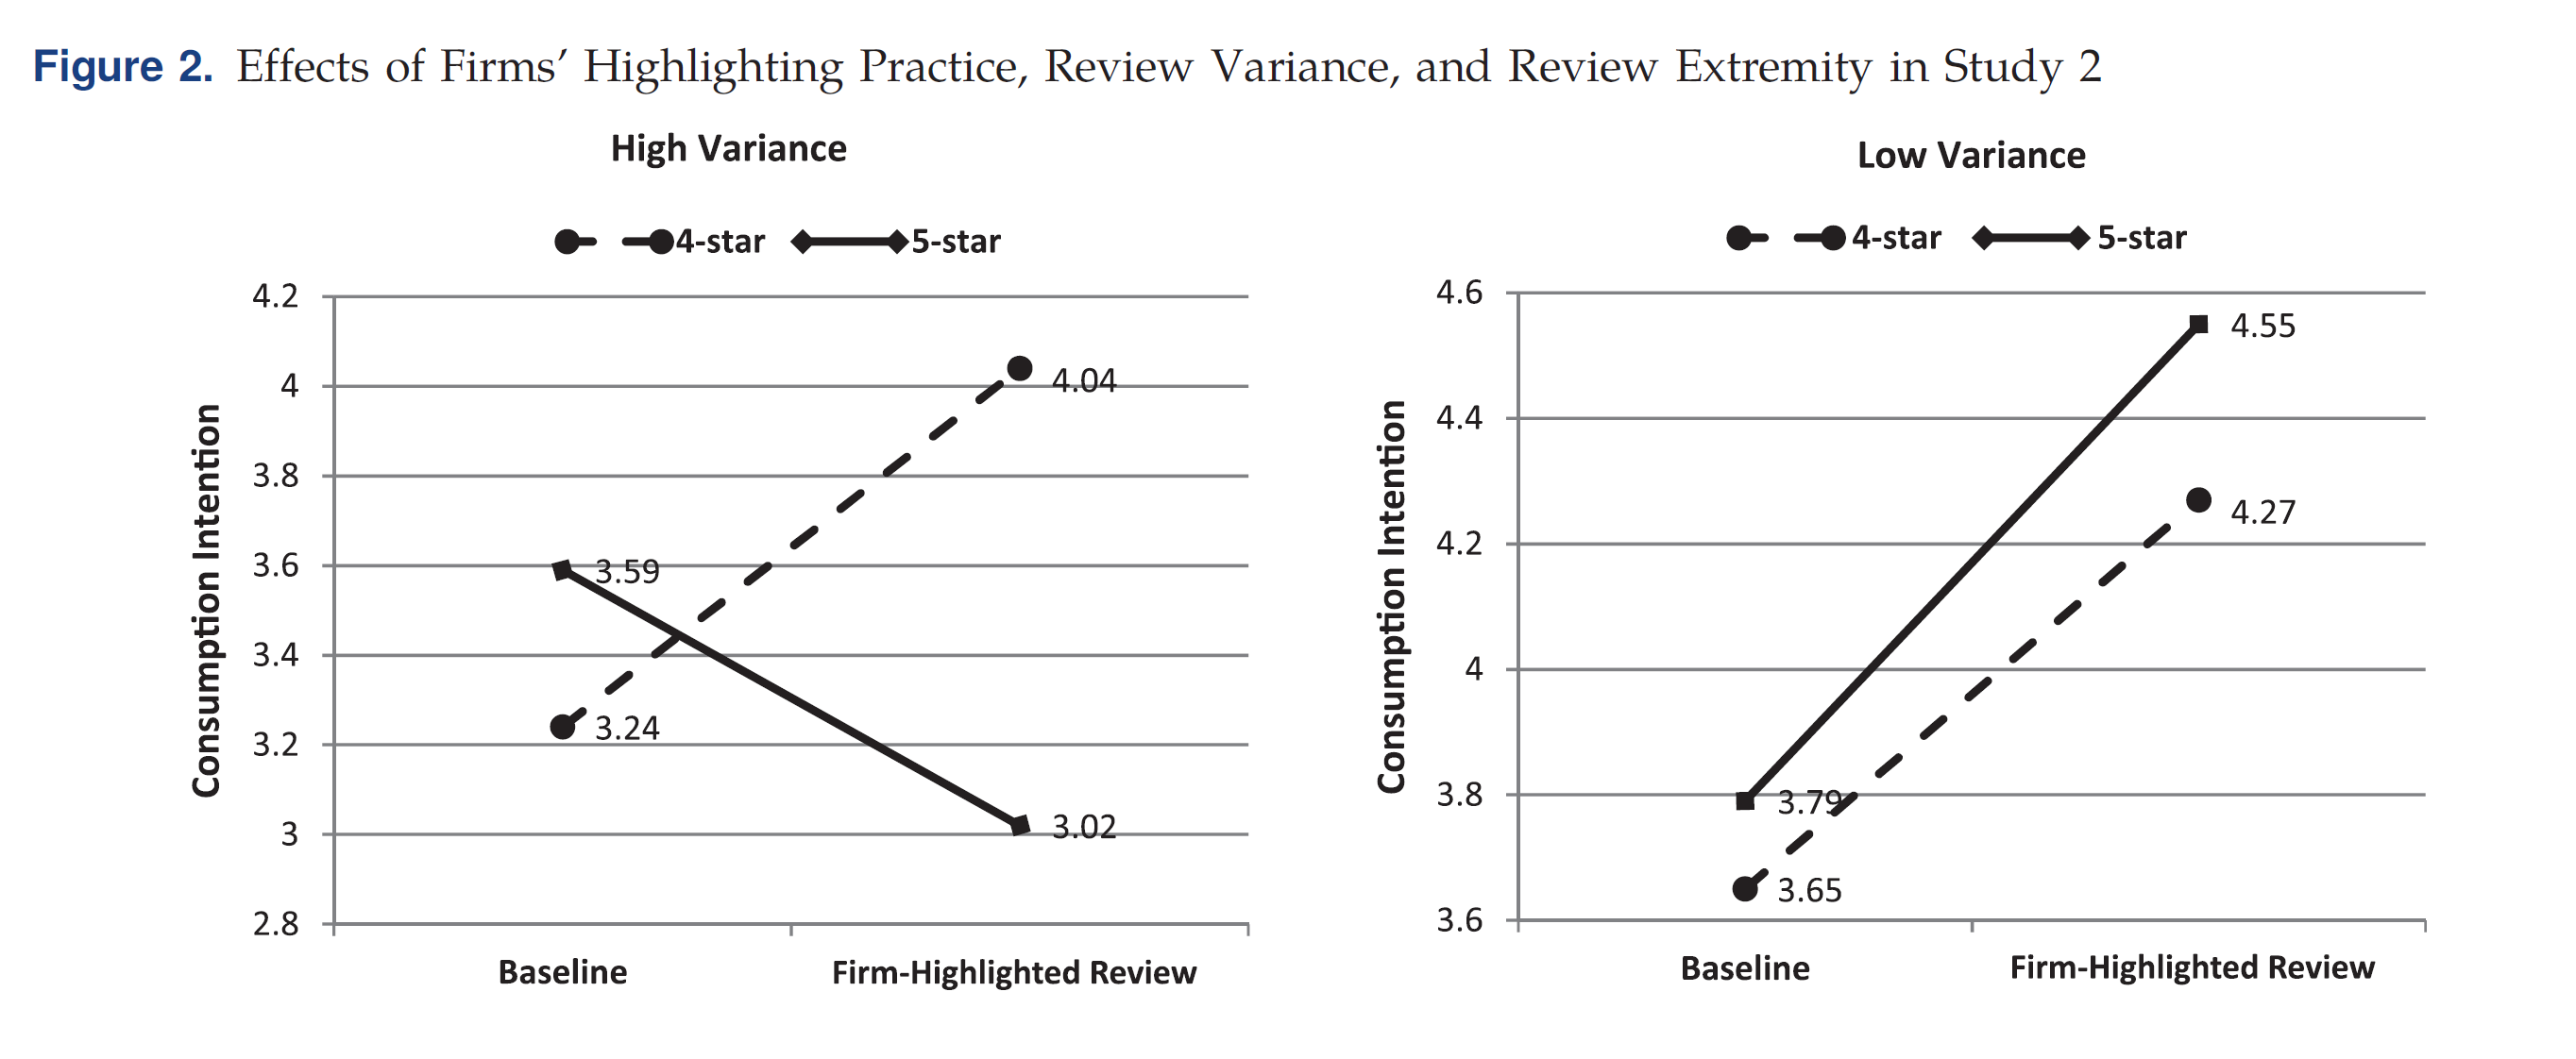
\includegraphics[width=0.8\linewidth]{pre04-imgs/pre04-2.png}
        \end{figure}

    \end{frame}

    \begin{frame}
        \frametitle{\textsc{Study II Discussion}}

        \begin{enumerate}
            \item In a moderately positive review context with high variance, using a less extreme, 4-star firm-highlighted review was more effective in inducing higher consumption intention.
            \item When the reviews tended to be homogeneously
            benign, using a 4-star or 5-star firm-highlighted review
            were both effective
            \item The interaction effect will largely disappear in a highly negative environment
        \end{enumerate}

    \end{frame}

    \subsection[\textsc{Study III}]{\textsc{Study III: Review Extremity and Firm's Reputation}}

    \begin{frame}
        \frametitle{\textsc{Source Characteristics - Firm's Reputation}}

        \textrm{\bfseries Hypothesis 3} For firms with mediocre reputations, the effect of using a positive but less extreme firm-highlighted review on increasing consumers' consumption likelihood is stronger than the effect of using an extremely positive firmhighlighted review;

        such a pattern will be weakened for firms with good reputations.

    \end{frame}

    \begin{frame}
        \frametitle{\textsc{Study III Design}}

            \begin{enumerate}
                \item Sample: working adults in a large city in China recruited by the research platform
                \item Focal business: a company that provided English language training for adults
                \item Reputation: \textbf{Good} - a leading company in the industry with a vision of contributing to the language education industry and to the society; \textbf{Mediocre}: a relatively new and with a modest market share

                \item Matrix:
            \end{enumerate}

            \begin{table}
                \scriptsize
                \begin{tabular}{c|c|c}
                    \toprule
                    Control & Extremity & Reputation \\
                    \midrule
                    Highlight & 5-star & Good \\
                    Baseline & 4-star & Mediocre \\
                    \bottomrule
                \end{tabular}
            \end{table}

    \end{frame}

    \begin{frame}
        \frametitle{\textsc{Study III Result}}

        \begin{figure}
            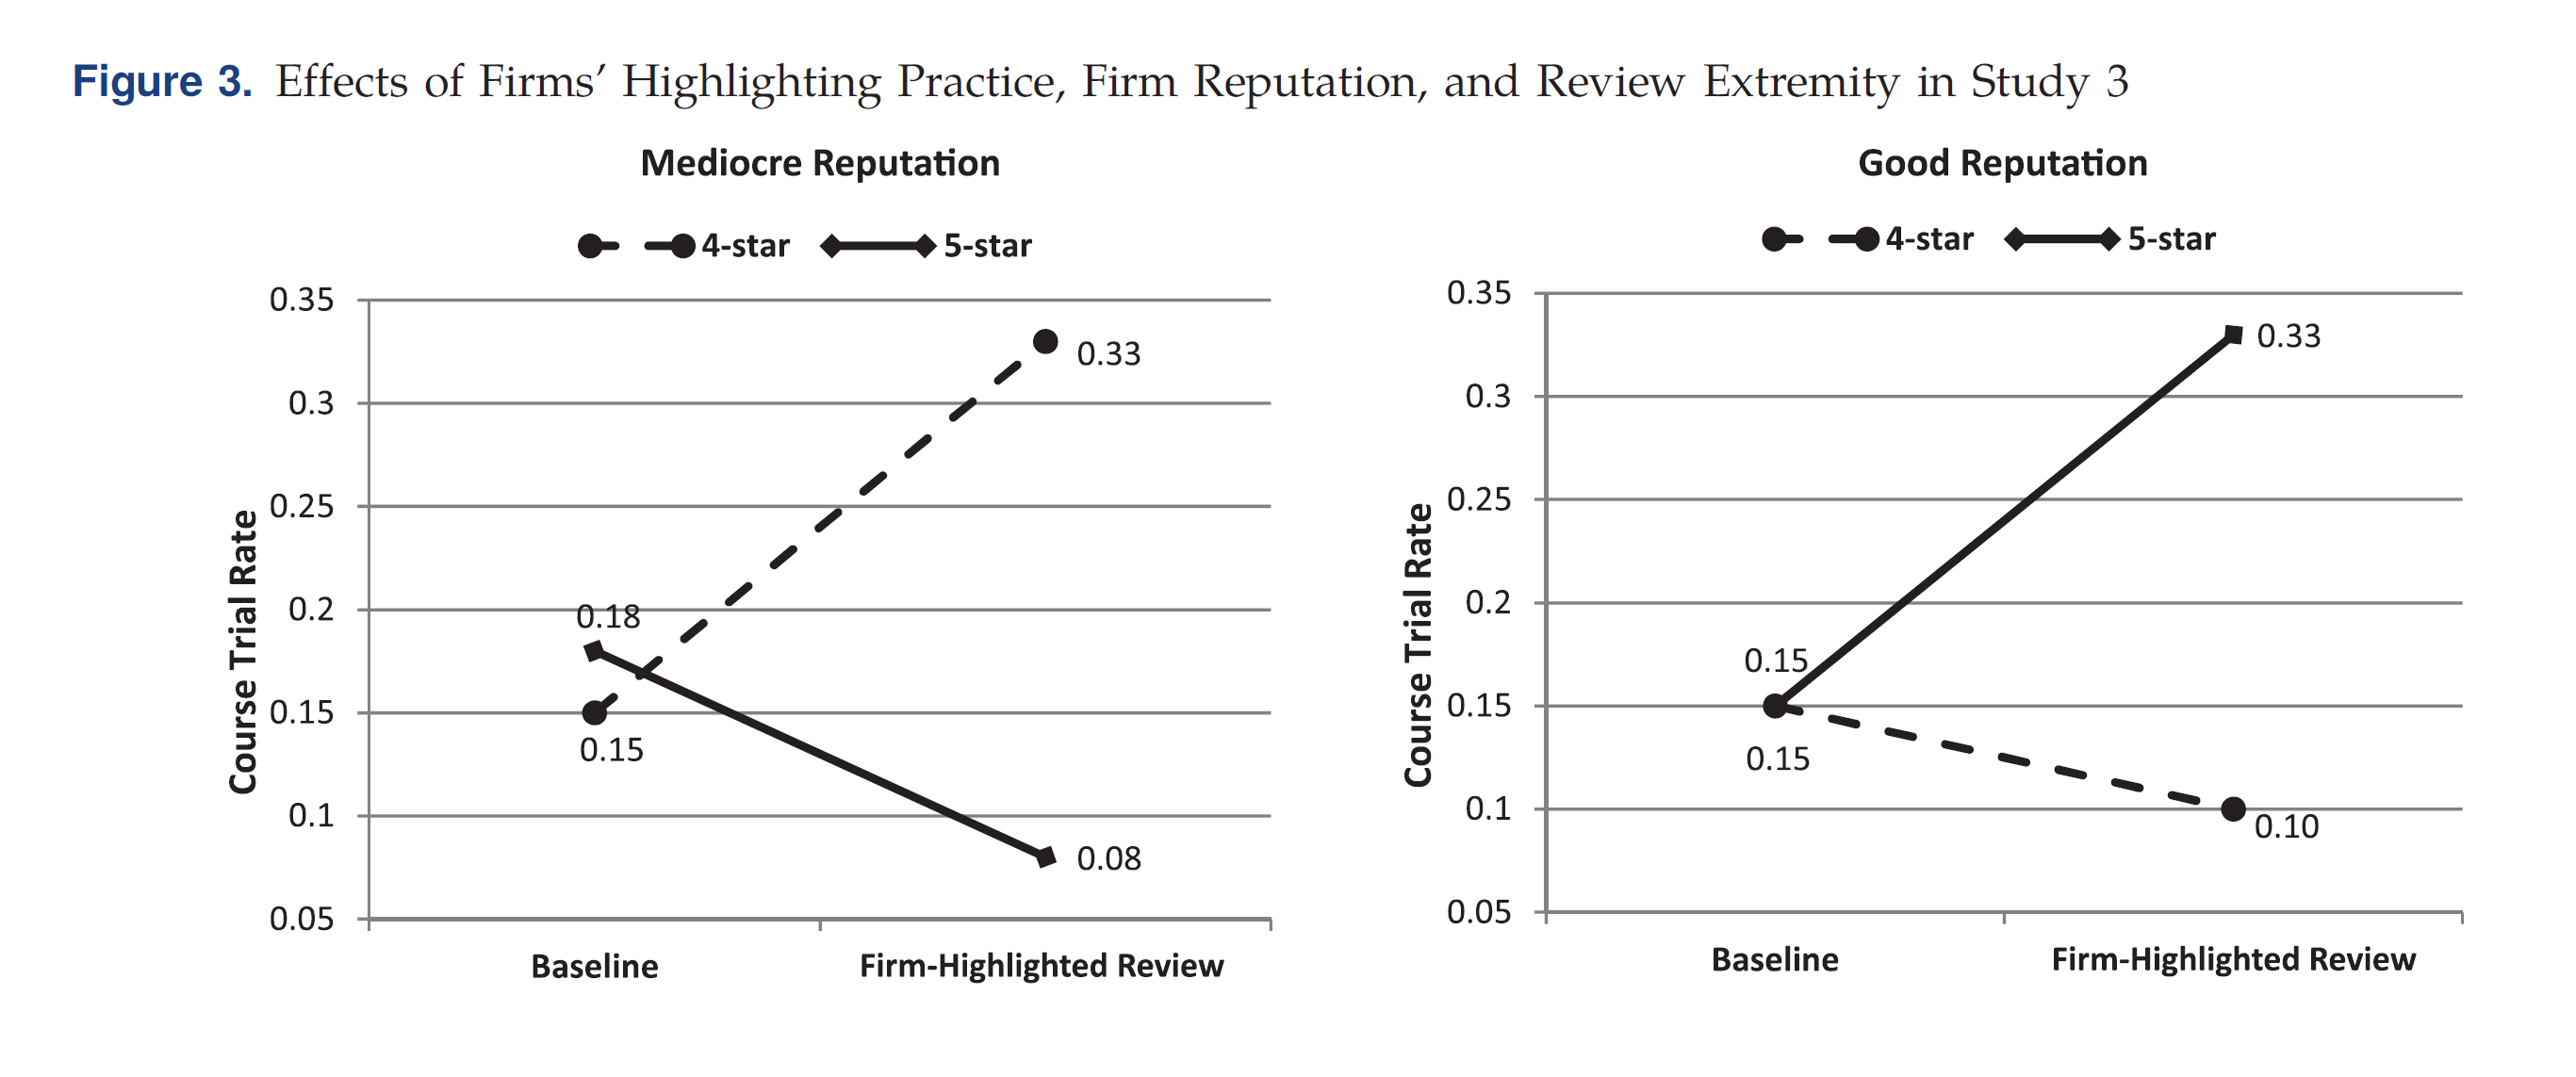
\includegraphics[width=0.8\linewidth]{pre04-imgs/pre04-3.png}
        \end{figure}

    \end{frame}

    \begin{frame}
        \frametitle{\textsc{Study III Discussion - Manipulation Check}}

        \small
        \setstretch{1.1}

        \begin{itemize}
            \item Participants who read the good reputation descriptions perceived the firm as more reputable than those who read the mediocre reputation descriptions.
            \item When the firm had a higher reputation, rating extremity did not affect consumers' skepticism about the review, but in the case of lower reputation, the 4-star highlighted review led to lower skepticism than the 5-star highlighted review.
            \item Presenting a firm-highlighted review generally led to a greater number of registrations for the trial sessions than the baseline conditions

            \begin{enumerate}
                \footnotesize
                \item \textbf{Good reputation: } A less extreme (i.e., 4-star) firm highlighted review led to a greater number of registrations for the trial program than those in the baseline condition whereas the effect of an extremely positive (i.e., 5-star) firm-highlighted review was not evident.
                \item \textbf{Mediocre reputation: } A 5-star firm highlighted review led to more registrations than the baseline condition, but a 4-star firm highlighted review did not differ from the baseline condition.
            \end{enumerate}
        \end{itemize}

    \end{frame}

    \section{\textsc{Summary}}

    \subsection{\textsc{Research Summary}}

    \begin{frame}
        \frametitle{\textsc{Strength}}

        \setstretch{1.2}

        \begin{enumerate}
            \item Carefully designed model and experiment with a clear structure.
            \begin{itemize}
                \item both laboratory experiments in different countries and an online experiment to test the hypotheses;
                \item incorporates eye-tracking technique to provide objective attention data;
                \item a real personal information barrier in study 3.
            \end{itemize}
            \item Prospective research background.
            \begin{itemize}
                \item The tendency of data in variable forms.
            \end{itemize}
            \item Result fits intuition and psychological theories.
            \begin{itemize}
                \item Self-fulfilling prophecy.
            \end{itemize}
        \end{enumerate}

    \end{frame}

    \begin{frame}
        \frametitle{\textsc{Shortcomings \& Supplementary}}

        \setstretch{1.2}
        \small

        \begin{enumerate}
            \item The representativeness of the sample in study 3 would be questioned as they probably don't have a "real" need for English learning as they have a relative low income in Chinese major cities.
            \begin{itemize}
                \item For example the course price in New Oriental (新东方) is \textyen750 per hour.
            \end{itemize}
            \item Reputation metric used in study 3 might be controlled by other hidden variables.
            \begin{itemize}
                \item The reputation of firms in the research was described under different tendency, which could be misunderstanding.
                \item The reputation of firms is a fuzzy conception, for example, excellent service with expensive price or cost-effective.
            \end{itemize}
        \end{enumerate}

    \end{frame}

    \begin{frame}
        \frametitle{\textsc{Shortcomings \& Supplementary}}

        \begin{enumerate}
            \setcounter{enumi}{2}
            \item Extremity metric used in the research is too simple and straightforward. The extremity more relies on review text rather than score.
            \begin{itemize}
                \item Text review can reflect more factors including service quality, flavor of the dish and transportation convenience.
            \end{itemize}
            \item The research did not take the cross-impact of both review variance and firm reputation.
        \end{enumerate}

    \end{frame}

    \subsection{\textsc{Improvements and Future Research Interests}}

    \begin{frame}
        \frametitle{\textsc{Improvements and Future Research Interests}}

        \begin{enumerate}
            \item Consider adding skepticism as an intermediate variable
            \begin{itemize}
                \item During the demonstration process of the article, \textbf{skepticism}, which will affect consumers, has been used to finally affect the purchase intention. Finally, the index \textbf{purchase intention} was used in the experimental verification index.
                \item There is a certain difference in concept between the two. Whether \textbf{skepticism} can be used as an intermediary variable ?
            \end{itemize}
        \end{enumerate}

    \end{frame}

    \begin{frame}
        \frametitle{\textsc{Improvements and Future Research Interests}}

        \begin{enumerate}
            \setcounter{enumi}{1}
            \item Apply mechanics of skepticism under different business scenarios including online newsfeed.
            \begin{itemize}
                \item Exaggerate descriptions used in misleading news.
                \item Content evaluation and supervision in social media.
            \end{itemize}
        \end{enumerate}

    \end{frame}
\end{document}